\chapter{Perception}

\section{Perception of luminance is not linear}
\begin{itemize}
\item The human eye perceives brightness differences non-linearly.
\item At low luminance, the eye is very sensitive (small changes in
  brightness are perceptually big).
\item At high luminance, the eye is less sensitive (bigger brightness
  jumps are needed to recognize a change in the luminance).
\end{itemize}

\section{Perception of the luminance VS the luminance}
\begin{itemize}
\item The perception of the intensity is not linear \cite{wikipedia_lightness}.
\end{itemize}
\begin{center}
  
\includegraphics[width=0.9\textwidth]{linear2}\\
  (In each row and column, the gradient is linear.)
\end{center}

\section{Perception of the luminance VS the frequency}
\begin{itemize}
\item The perception of a change of the intensity varies with the spatial frequency.
\end{itemize}
\begin{center}
  
\includegraphics[width=0.65\textwidth]{CSF3}\\
  (\gls{CSF}.)
\end{center}

\section{Perception of the \popup{luma}{Luminance.} VS the neighborhood}
\begin{itemize}
\item The perception of the intensity depends the neighbour pixels.
\end{itemize}
\begin{center}
  
\includegraphics[width=0.8\textwidth]{linear3}\\
  (In each block, all the pixels have the same intensity.)
\end{center}

\section*{}
\begin{itemize}
\item The perception of the intensity depends the neighbour pixels.
\end{itemize}
\begin{center}
  
\includegraphics[width=1.0\textwidth]{contraste_simultaneo}\\
  (All the internal squares have the same intensity.)
\end{center}

\section{Perception of the luma VS the visualization time}
\begin{itemize}
\item The perception of the intensity depends the visualization time.
\end{itemize}
\begin{center}
  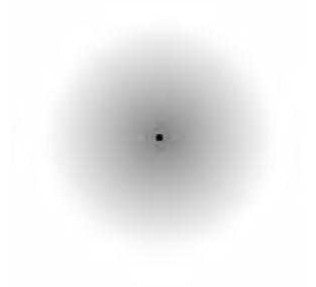
\includegraphics[width=0.4\textwidth]{punto_y_difuminado}\\
  (Look to the central point for a while.)
\end{center}

\section{Noise masking}
\begin{itemize}
\item The perception of the structures depends on the type and intensity of the noise.
\end{itemize}
\begin{center}
  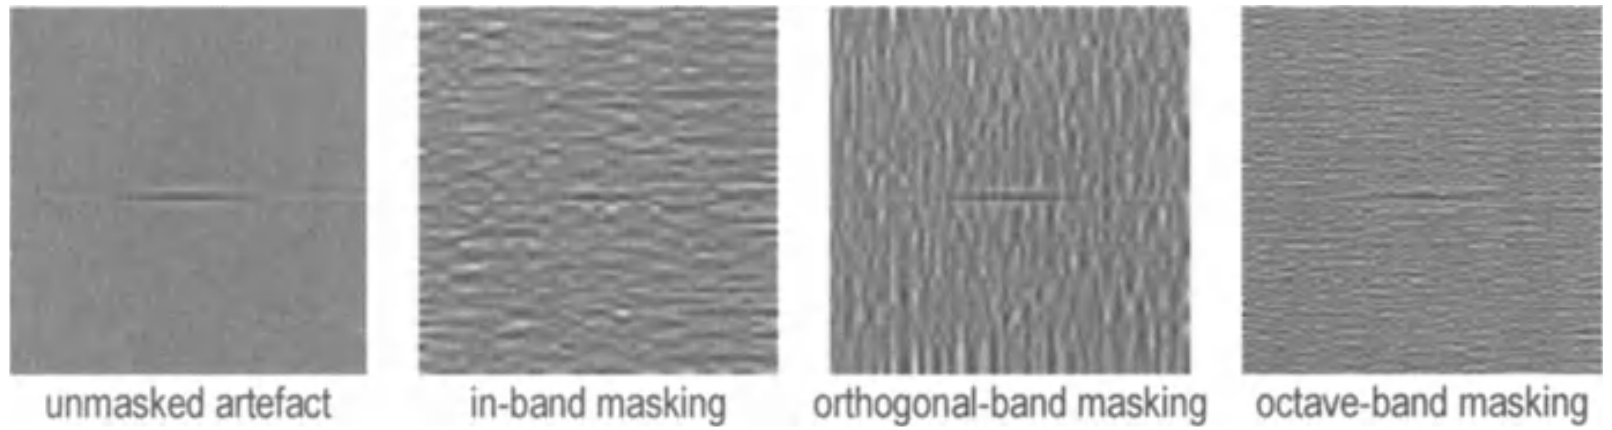
\includegraphics[width=1.0\textwidth]{noise_masking}\\
  (Different effects of Gaussian noise in the Wavelet domain.)
\end{center}

\section{Retinex theory}

Retinex theory was introduced by Edwin Land (the founder of Polaroid)
to explain human color perception. The name comes from retina + cortex
— highlighting that perception is not purely a retinal process but
involves cortical processing too.
